\documentclass[14pt]{mmcs_article}
\usepackage[russian]{babel}
\usepackage{amsmath, amsthm, amsfonts, amssymb}

%\graphicspath{{images/}}%путь к рисункам

\begin{document}

%см. РЕКОМЕНДАЦИИ ПО ОФОРМЛЕНИЮ
%И ПРЕДСТАВЛЕНИЮ КУРСОВЫХ И ВЫПУСКНЫХ %КВАЛИФИКАЦИОННЫХ РАБОТ СТУДЕНТОВ ИНСТИТУТА %МАТЕМАТИКИ, МЕХАНИКИ И КОМПЬЮТЕРНЫХ НАУК


% ----------------------------------
% Внимание!
% Изменяйте только строки, перед которыми стоят знаки комментариев
% ----------------------------------

\thispagestyle{empty}
\begin{singlespacing}
    \begin{center}

        МИНОБРНАУКИ РОССИИ\\ [12pt]
        Федеральное государственное автономное образовательное\\
        учреждение высшего образования\\
        <<Южный федеральный университет>>

        \vspace{\baselineskip}
        Институт математики, механики\\
        и компьютерных наук им.~И.\,И.~Воровича


        \vfill
        % Фамилия Имя Отчество студента
        \textbf{Яценко Артём Алексеевич}

        \vspace{15mm}
        %НАЗВАНИЕ РАБОТЫ должно полностью соответствовать 
        % приказу по ЮФУ (для выпускных квалификационных работ)
        {\bf АВТОМАТИЗАЦИЯ СОПОСТАВЛЕНИЯ \\
            РЕЗЮМЕ И ВАКАНСИЙ}

        \vspace{15mm}
        ВЫПУСКНАЯ КВАЛИФИКАЦИОННАЯ РАБОТА\\
        по направлению подготовки\\
        % Направление обучения 
        02.04.02~-- Фундаментальная информатика и информационные технологии

        \vspace{10mm}
        \textbf{Научный руководитель~--}\\
        % указать данные о руководителе
        % должность, степень, звание Фамилия Имя Отчество
        доц., к.\,ф.-м.\,н. Юрушкин Михаил Викторович

        \vspace{7mm}
        \textbf{Рецензент~--}\\
        % указать данные о рецензенте
        % должность, степень, звание Фамилия Имя Отчество
        доц., к.\,т.\,н. ОТСУТСТВИЕ РЕЦЕНЗЕНТА


        \vspace{15mm}

        \noindent
        % указать Фамилию и инициалы руководителя
        % образовательной программы
        \begin{flushleft}
            Допущено к защите:\\
            руководитель \\
            образовательной программы \underline{\hspace*{60mm}} Демяненко Я.\,М.
        \end{flushleft}




        \vfill
        % год!
        Ростов-на-Дону -- 2025

    \end{center}

    \singlespacing
\end{singlespacing}% для работы магистра

\renewcommand{\contentsname}{Оглавление}

\tableofcontents

%=======================
\newpage
\addcontentsline{toc}{section}{Постановка задачи}

\section*{Постановка задачи}


В постановке задачи коротко (по пунктам) указывается, что необходимо сделать в рамках работы. Раздел <<Постановка задачи>> должен соответствовать заданию на курсовую или выпускную квалификационную работу, подписанному научным руководителем.

%=======================
\newpage
\addcontentsline{toc}{section}{Введение}
\section*{Введение}

Введение должно содержать общее описание предметной области и решаемой задачи, указание на используемые методы решения, возможно, на существующие альтернативные подходы к решению. Из введения должно быть ясно, чему посвящена работа.

Большинство рекомендаций были взяты из работы \cite{stud:b0}, в~котором
содержатся подробные рекомендации по оформлению
и представлению курсовых
и выпускных квалификационных работ.




%=======================
\newpage
\section{Описание полученных результатов}\label{dsfs}

В основной части работы должны быть описаны полученные результаты. Здесь возможны:
\begin{itemize}
  \item определения основных понятий, систематизация имеющихся точек зрения по изучаемому вопросу, аргументированная формулировка собственной точки зрения;
  \item теоретические и экспериментальные результаты, полученные автором;
  \item детальные описания методов и алгоритмов решения задач и фактов, лежащих в их основе;
  \item описания разработанных программ, включая образцы экранных\linebreak форм и фрагменты кода.
\end{itemize}

Помимо изложения результатов работа должна содержать методы их получения (доказательства теорем, методика проведения экспериментов, обоснования корректности алгоритмов, и т.\,п.).

В основном тексте также допустимо указывать результаты работы программ, если они имеют небольшой объём. В противном случае эти результаты (или их часть, не вошедшая в основной текст) могут быть приведены в приложениях.


Переносы в заголовках разделов не допускаются.

Необходимо обращать внимание на написание дефисов, длинных и коротких тире в основном тексте, например:

\emph{Одним из участников Великой Отечественной войны и парада Победы на Красной площади в~1945 году был выдающийся российский учёный, чьё имя с гордостью носит наш Институт, и чью столетнюю годовщину со дня рождения мы будем торжественно отмечать 21 июня~--- Иосиф Израилевич Ворович (1920--2001).}


\subsection{Рекомендуемые объёмы работ}

Рекомендуемые объёмы работ приведены в~табл.\,\ref{stud:table:1}. В~скобках указаны рекомендуемые объемы для работ в~области педагогического образования.

\begin{table}[H]
  \centering

  \caption{Рекомендуемые объёмы работ}\label{stud:table:1}

  \begin{tabular}{|p{85mm}|c|}
    \hline
    \multicolumn{1}{|c|}{\bf Уровень работы} &
    \multicolumn{1}{c|} {\bf Объём (в страницах)}              \\
    \hline
    Курсовая работа                          & 8--10 (15--20)  \\
    \hline
    Выпускная квалификационная работа\newline
    (4 курс бакалавриата)                    & 15--20 (40--50) \\
    \hline
    Выпускная квалификационная работа\newline
    (2 год магистратуры)                     & 40--50 (50--70) \\
    \hline
  \end{tabular}
\end{table}



\subsection{Вставка изображений и таблиц}

Все таблицы, рисунки, схемы, диаграммы и другие объекты, вставляемые в текст, должны быть пронумерованы, подписаны и выровнены по центру, в~тексте должна присутствовать ссылка на них (рис.\,\ref{stud:fig:1}).


\begin{figure}[H]
  \centering
  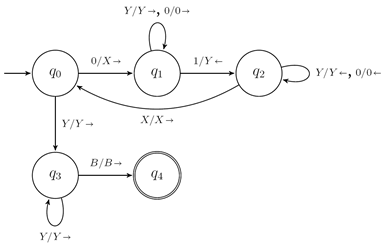
\includegraphics[scale=1.2]{Fig_T.png}
  \caption{Диаграмма переходов машины Тьюринга}\label{stud:fig:1}
\end{figure}


\subsection{Фрагменты исходного кода}

Для иллюстрации излагаемого материала в основной текст можно вставлять фрагменты исходного кода (тексты программ). Они должны быть набраны моноширинным шрифтом (например, \texttt{Courier New}), 12~пунктов, с~одинарным интервалом и выравниванием по левому краю. Если к~фрагментам кода требуется указывать ссылки, их тоже надо снабжать заголовками, как в~случае листингов~\ref{stud-lst:1}--\ref{stud-lst:3}, приведенных ниже.

Если строка кода не помещается на одну строку страницы, её следует разбивать на части в соответствии с принятым стилем форматирования кода, а не автоматически. Размер непрерывных фрагментов исходного кода не должен превышать половины страницы. Фрагменты большего размера следует помещать в приложении к работе.


\subsubsection{Примеры фрагментов кода}

Ниже приведены листинги с заголовками.

\begin{lstlisting}[language=C++, caption={C++, пример кода}, label=stud-lst:1]
#include <iostream>
int main()  // однострочный комментарий
{
  std::cout << "Привет, мир!" << std::endl;
}
\end{lstlisting}


\begin{lstlisting}[language=Python, caption={Python, пример кода}, label=stud-lst:2]
print("Привет, мир!")  # comments
\end{lstlisting}

\begin{lstlisting}[language=TeX, caption=\LaTeX, label=stud-lst:3]
% параметр language в наших листингах только для себя
\bf Привет, мир!
\end{lstlisting}



%=======================
\newpage
\section{Примеры оформления формул}

Внутритекстовая формула
$ \int\limits_a^b f(x)\,dx$ не всегда выглядит красиво даже в \LaTeXe.

Но формулы, вынесенные в отдельную строчку всегда выглядят шикарно
\[
  \lim_{d\to 0} S_n =
  \int\limits_a^b f(x)\,dx.
\]

Для того чтобы {\TeX} автоматически мог ссылаться на нумеруемые формулы нужно указывать команду \verb"\label"
\begin{equation}\label{eq:1}
  \frac{abc}{xyz}.
\end{equation}
Формула (\ref{eq:1}) была оформлена с помощью окружения \textsf{equation}.

%=======================
\newpage
\addcontentsline{toc}{section}{Заключение}
\section*{Заключение}

Заключение должно содержать информацию о проделанной работе и полученных результатах.

При написании текста работы следует иметь в виду, что её цель состоит в том, чтобы продемонстрировать квалификацию автора. Поэтому следует избегать общих и, тем более, тривиальных или нравоучительных высказываний. Мотивация выполняемой работы не должна носить слишком конкретный характер. Во время выступления на защите желательно избегать упоминаний об особенностях стандартных компонентов пользовательского интерфейса программ (<<нажимаем на правую кнопку>>, <<перетаскиваем фрагмент мышью>> и т.\,д.). Не следует комментировать задаваемые после защиты вопросы. Ответы на вопросы должны быть краткими.



%=======================
\newpage

\addcontentsline{toc}{section}{Литература}
\renewcommand{\refname}{\centering \textbf{Литература}}

\begin{thebibliography}{0}
  \bibitem{stud:b0}
  Рекомендации по оформлению
  и представлению курсовых
  и выпускных квалификационных работ
  студентов института математики,
  механики и компьютерных наук.~--
  Ростов н/Д, 2020.

  \bibitem{stud:b1}
  Жуков М.\,Ю., Ширяева Е.\,В.
  \LaTeXe: искусство набора и вёрстки текстов с~формулами.~-- Ростов н/Д : Изд-во ЮФУ, 2009.
\end{thebibliography}



\end{document}
% ----------------------------------------------------------------


\lstset{ %
  language=C++,                 % выбор языка для подсветки (здесь это С++)
  basicstyle=\small\sffamily, % размер и начертание шрифта для подсветки кода
  numbers=left,               % где поставить нумерацию строк (слева\справа)
  numberstyle=\tiny,           % размер шрифта для номеров строк
  stepnumber=1,                   % размер шага между двумя номерами строк
  numbersep=5pt,                % как далеко отстоят номера строк от подсвечиваемого кода
  backgroundcolor=\color{white}, % цвет фона подсветки - используем \usepackage{color}
  showspaces=false,            % показывать или нет пробелы специальными отступами
  showstringspaces=false,      % показывать или нет пробелы в строках
  showtabs=false,             % показывать или нет табуляцию в строках
  frame=single,              % рисовать рамку вокруг кода
  tabsize=2,                 % размер табуляции по умолчанию равен 2 пробелам
  captionpos=t,              % позиция заголовка вверху [t] или внизу [b]
  breaklines=true,           % автоматически переносить строки (да\нет)
  breakatwhitespace=false, % переносить строки только если есть пробел
  escapeinside={\%*}{*)}   % если нужно добавить комментарии в коде
  extendedchars=true,
  commentstyle=\color{mygreen},    % comment style
  stringstyle=\bf,
  commentstyle=\ttfamily\itshape,
  keepspaces=true % пробелы между русскими буквами
  aboveskip=3mm,
  belowskip=3mm

}


\renewcommand\NAT@bibsetnum[1]{\settowidth\labelwidth{\@biblabel{#1}}%
  \setlength{\leftmargin}{\bibindent}\addtolength{\leftmargin}{\dimexpr\labelwidth+\labelsep\relax}%
  \setlength{\itemindent}{-\bibindent+\fivecharsapprox}%
  \setlength{\listparindent}{\itemindent}
  \setlength{\itemsep}{\bibsep}\setlength{\parsep}{\z@}%
  \ifNAT@openbib
    \addtolength{\leftmargin}{\bibindent}%
    \setlength{\itemindent}{-\bibindent}%
    \setlength{\listparindent}{\itemindent}%
    \setlength{\parsep}{0pt}%
  \fi
}
\renewcommand{\thesection}{\arabic{section}.}
\renewcommand{\thesubsection}{\arabic{section}.\arabic{subsection}.}
